% !TeX root = ../main.tex

\begin{survey}
\label{cha:survey}

\title{Survey on Graph Generation}
\maketitle

Graphic data that includes nodes and edges shows everywhere in our life.
For example, friendship between people and interactions on social
networks, citation of papers, and activities like transferring accounts
in the financial field can be modeled with graphs. Using graphs to do
analysis and research is popular, so graph data plays an important role
and is the basis of this field.

Graphic data generation is an important issue, and synthetic datasets
are widely used in research. When we find an algorithm, we need to do
experiments on different scales and different types of datasets.
Usually, it is not enough to use real datasets only. On the one hand,
the number of public datasets is small. On the other hand, the size of a
dataset is decided by its data, we can find it difficult to get
extremely large scale real-world social graphs. So we need to generate
new data or expand from the existing data to obtain data that we needed,
usually of the same distribution and different sizes. Therefore,
synthetic datasets are a good choice for researchers.

Among the generating methods for synthesizing datasets, there are
rule-based methods for graph generation, and there are also some
algorithms for graph generation based on a given graph's pattern.

There are two points to consider: the similarity between synthetic
datasets and real data, and the efficiency of the generation method.
Over the past decades, many researchers have focused on the problem and
have made in-depth research based on the characteristics of real graphs.
It includes some traditional methods based on distribution and
probability theory, and there are also some methods based on neural
networks.

Most of the generation methods are for static graphs, but generation of
dynamic graphs has also been studied by some researchers. Dynamic graphs
can be seen as the time series of graphs, so they're more difficult to
generate.

\section{Traditional Methods}

These methods are based on the priori structural assumptions from the
observation of social networks, such as power law, small-world property,
the community structure of social networks. We can use pieces of
knowledge from probability theory and some result of distribution from
the real-world to generate nodes, edges as well as attributes. In these
methods, some optimization steps are introduced to speed up the process
of generation.

Here are two of this kind of method, S3G2 and FastSGG.

\subsection{S3G2\cite{Minh2012S3G2}}

“S3G2” is short for “Scalable Structure-correlated Social Graph
Generator”, it is a generator that can produce scalable a social network
graph which is structure-correlated. So-called “structure-correlated” is
not the attributes of a single node or the community-structure we
usually talk about, it mainly focuses on the way nodes happen to be
connected, which is the edges of the graph based on the nodes'
attributes or labels.

It's a novel graph generator that can take node attribute similarity
into account when generating edges of a graph. It can keep similar graph
connectivity features known in real social networks, which can be an
important factor in the performance of graph algorithms so that it can
produce graphs suitable for the testing process of many graph
algorithms.

It also has the ability to scale up in parallel, allowing large-scale
results to be generated quickly on clusters.

\subsubsection{Method Ideas}

In a social network, the distribution and characteristics of nodes and
edges in a graph are related to previously generated nodes, edges, and
the attributes of them. For example, people from different countries
have different names. Another example is that people who attend the same
university at the same time are more likely to become friends.
Therefore, it is necessary to consider node attributes and their
associated distribution for graph generation, but other graph generators
did not consider this before this paper was published.

The generation period of S3G2 is divided into several stages, each of
which revolves around a correlation dimension. A method called MapReduce
is also used to reduce disk I/O pressure so that it can generate larger
data graphs.

In the algorithm, the attribute information of the nodes needs to be
assigned, and the probability of edges between the two nodes can be
derived from their attributes.

\subsubsection{Formal Definition}

Class and dictionary information is introduced in the graph generated by
S3G2, so this graph is different from the concept of the graph we
usually define. In this graph, besides representing the relationship
between two instances through edges, an instance has certain attributes
in the form of edges. So there are two kinds of edges, one of them shows
the connection of objects, the other points the object to its attribute
info; there are also two kinds of nodes, one of them is an object and
the other is the attribute value.

Formally, the graph is represented as \(G(V, E, P, C)\). Where:

\begin{itemize}
\item
  \(C\) denotes a collection of classes;
\item
  \(V\) denotes a node, possibly a text or an instance of a class,
  \(V=L \cup \bigcup_{c \in C} O^{c}\), where \(L\)denotes a collection
  of all text, \(O^c\)denotes an instance belonging to category \(C\);
\item
  \(P\) denotes attributes,
  \(P=\left\{P^{L(x)} | \forall x \in C\right\} \cup\left\{P^{E(x, y)} | \forall x, y \in C\right\}\),
  where \(P^{L(x)}\) denotes the set of text attributes for the category
  \(x\), and \(P^{E(x,y)}\) denotes the set of attributes from category
  \(x\)to the edge of the category \(y\);
\item
  \(E\) denotes an edge, denoted by a tuple of three,
  \(E=\left\{\left(n_{1}, n_{2}, p\right) | n_{1} \in O^{x} \wedge\left(\left(n_{2} \in L \wedge p \in P^{L(x)}\right) \vee\left(n_{2} \in O^{y} \wedge p \in P^{E(x, y)}\right)\right)\right\}\),
  which can indicate that an instance has some attribute, or that there
  is a relationship between two instances and the attributes of that
  relationship are given. There are the following two cases:
\item
  \(n_1\) (an instance of the class \(x\)) has an attribute named \(p\)
  which is \(n_2\);
\item
  There is a relationship between \(n_1\) (it's an instance of the class
  \(x\)) and \(n_2\) (it's an instance of the class \(y\)), it has the
  attribute \(p\).
\end{itemize}

\vspace{0.2cm}

S3G2 also introduced the concept of a dictionary for each attribute
\(l\in P^{L(x)}\), specifying structure \(PD_l(D, R, F)\) for a
dictionary that has a corresponding attribute \(l\). Here \(D\) denotes
a dictionary, \(R\) for a sorting function, \(F\) for a probability
density function, these are defined as follows:

\begin{itemize}
\item
  Here the dictionary \(D\) is a set of length \(|D|\),
  \(D=\{v_1,., v_{|D|}\}\);
\item
  \(R\) is a bijection from \(D\) to \(\{1,.,|D|\}\), which gives each
  value in the dictionary order. (To save storage space, S3G2 actually
  set an order threshold of \(N\), where the top-N values in the
  dictionary are stored, but the rest of the values are assigned a
  random order);
\item
  \(F\) is a probability density function, which takes an order
  \(\{1,.,|D|\}\) to \([0,1]\) and gives the probability for each order.
  The cumulative distribution function \(F'=\sum\limits_{i=1}^r F(i)\)
  is also introduced in this paper.
\end{itemize}

\vspace{0.2cm}

Because different attribute parameters can lead to different results, we
need to put this information in the above functions. For example,
\(R[z](c)\) denotes the sorted value of \(c\) based on the attribute
\(z\).

\subsubsection{Algorithm for Probability of Edges}

A simple method is to use a degree distribution of \(N(·)\) to determine
the degree of this node each time when we need to generate a new node in
a graph generation process. The distribution is typically a power-law
distribution (\(N(h)\sim \gamma \cdot h^{-\lambda}\)). Under different
attributes, \(\gamma\) and \(\lambda\) may be different, so the
attribute information can be used to determine the degree distribution
parameters of a node in S3G2.

However, the practice of only using this method can result in a smaller
graph, which usually contains isolated submaps or have tree structures
with only a few layers.

In order to generate large-scale, highly connected graphs in a better
method, we need to consider how edges are generated after a generation
action finished for a batch of nodes. Because the attributes of a node
affect how many neighbors it may have and how the nodes connect, this
computation of this can be expensive. Therefore, S3G2 simplified the
calculation by using correlation dimensions, which represent the
probability of connections between nodes with their attributes as
follows:

\begin{itemize}
\item
  Given two types of nodes, \(O^x\) and \(O^y\), the attributes of the
  edges between the two types, \(e\in P^{E(x, y)}\), we can define the
  correlation dimension, \(CD_e(M^x, M^y, F)\). Here are two similarity
  functions, \(M^x, M^y\). And \(F\) is a probability distribution
  function.
\item
  The similarity function \(M\) converts each node into a number. After
  all the nodes have been calculated, they can be sorted using these
  numbers to determine the similarity between the nodes by their
  distance calculated by the order information.
\item
  For many social network data, we consider the connection of the same
  category (e.g. people). In this condition, \(x=y\), \(M^x=M^y\).
\item
  \(F\) is a function which accepts the difference of the order between
  one node and another node, and can output the probability of
  connection between the two nodes. For more efficient calculations, the
  number of input values has an upper limit of \(W.t\), which means that
  each node only considers connecting to nodes within the distance
  \(W.t\), which is some of the most similar nodes. This upper limit,
  \(W.t, \) is called window length because it is equivalent to
  considering only the information of subsequent nodes of that length
  (within a window) each time when the program considers the node's
  adjacency.
\end{itemize}

\vspace{0.2cm}

After getting the edges between nodes between which the distance is no
more than \(W.t\) according to the relevant dimensions, we can generate
some other edges for all the nodes without considering their distance,
using a pure random probability function.

\subsubsection{MapReduce}

This is an algorithm that enables S3G2 to support parallelism:

\begin{itemize}
\item
  The map function can be run in parallel on a cluster to process input
  data and the result will be returned with an additional key;
\item
  According to the generated key, the result will be sent to different
  reducers;
\item
  The key can be used to sort the data to get the similarity between
  them;
\item
  The reduce function processes this stream of data. Similar data can be
  processed in the same reducer. Here, we will sort the correlation
  dimensions and generate the edges by using the method of the sliding
  window.
\end{itemize}

\vspace{0.2cm}

As mentioned before, when the correlation dimensions are used to process
data, the method called sliding window is used. The sliding window will
slide on the sorted nodes and generate the edges between the similar
nodes. Because only similar data is considered, it can be divided into
multiple operations on different reducers.

Because there are different attributes, MapReduce must be operated every
time in every different correlation dimensions. Another issue to
consider is the order of dependencies. Due to the dependency between
different attributes and nodes, it is necessary to consider the
dependent relationship first. For example, if we need to generate chats
or comments between friends, we need to first consider the generation of
a friend relationship, then consider the generation of comments.

\subsection{FastSGG\cite{FastSGG}}

FastSGG is a configurable social graph generator which can generate
trillion-scale social graphs efficiently. In the generation process,
social network features are taken into account. Users can specify some
characteristics of the graph, which can be flexibly adapted to many
different scenarios. The generated graphs have some known social network
characteristics, such as small-world, power-law degree distribution,
community structure, and has advantages in generation efficiency and
scalability.

An efficient Degree Distribution Generation model (\(D^2G\)) is proposed
in this paper. There are two basic steps in the process of graph
generation: determination of out-degree for a source vertex and
determination of a target vertex to construct an edge. In the \(D^2G\)
model proposed in the paper, it only takes \(O(1)\) to determine the
degree and each target vertex each time, so it is a suitable model for
large-scale map generation.

The methods presented in this paper are not limited to the power-law
distribution. For any distribution, \(D^2G\) can be used to generate
vertices if either probability density function (PDF, defined for
continuous variables) or probability mass function (PMF, defined for
discrete variables) is given.

\subsubsection{Schema Definition}

A graph is represented in the form of \(G=(V, E)\) in FastSGG. Each
vertex \(v\) in \(V\) is a tuple of three, which can be written in the
form of \((id, lbl, attr)\). Each edge \(e\) in \(E\) can be written in
the form of an edge tuple \((v_s,  v_t, lbl, attr)\). In both vertex
tuples and edge tuples, \(lbl\) denotes a label, which we can also find
in the schema definition; \(attr\) is attributes that are represented as
a set of key-value pairs.

We can define the schemas of vertices, edges, and community as follows:

\begin{itemize}
\item
  Vertex schemas are expressed in the form of
  \(VS = (lbl, amount, attr)\). This triple means we want to generate
  nodes labeled \(lbl\), the total amount of which is \(amount\) and the
  attribute information is provided in \(attr\);
\item
  Edge schemas can be expressed in the form of
  \(ES = (lbl, lbl_s, lbl_t, amount, distr_{in}, distr_{out}, attr)\),
  which indicates that we want to generate edges labeled \(lbl\), the
  total amount of which is \(amount\), which are from vertices labeled
  \(lbl_s\)and the target vertices are labeled \(lbl_t\). In-degree
  distribution of target vertices and out-degree distribution of source
  vertices are \(distr_{in}\) and \(distr_{out}\), respectively, and the
  attribute information is provided in \(attr\);
\item
  A community schema
  \(CS = (lbl_e, amount, \lambda_s, \lambda_t, \rho)\) shows that the
  community is labeled \(lbl_e\), and the total number of communities is
  \(amount\). The community size conforms to a power-law distribution,
  \(\lambda_s, \lambda_t\)denotes the power-law parameters of the
  community size in source and target vertices, respectively. \(\rho\)
  is the community fusion parameter, controls the number of edges
  between different communities. Larger \(\rho\) means that there will
  be more edges among communities.
\end{itemize}

\vspace{0.2cm}

\subsubsection{General Graph Generation}

We can use an adjacency matrix \(M\) of size \(n_s\times n_t\) to
represent the graph and \(M_{i,j}=1\) means there is an edge from
\(v_i\)to \(v_j\).

The generation process is a streaming process, each time for each node,
its output is derived from the probability distribution, and each target
vertex is determined from the distribution information so that we can
generate an edge. In the form of the matrix, we do the following things:

\begin{itemize}
\item
  For each row (each source vertex), we first determine how many 1s
  there will be by the determination of out-degree \(outd\);
\item
  Then we need to determine the target vertices. In other words, we use
  the algorithm to determine \(outd\) cells and fill in 1s.
\end{itemize}

\vspace{0.2cm}

These two steps are the edge generation process. We need to generate
random numbers that conform to a given probability distribution. Random
operations are performed here using the inverse of the cumulative
distribution function, which is \(F^{-1}\). We can generate a uniformly
distributed random number \(u\) in the range of \([0, 1]\) so that we
can use \(F^{-1}(u)\) to get a random number that conforms to the given
probability distribution.

\subsubsection{Social Graph Generation}

The significant difference between a social graph and a general graph is
that there are community structures in a social graph. Since communities
are such structures with groups of vertices densely connecting
internally and sparsely connecting externally, we can do a series of row
and column transformations on the adjacency matrix to make the vertices
of the same communities next to each other to get obvious block
structures on the main diagonal.

To generate connections between different communities, this paper uses
\(d_{out}(u)\) to express the out-degree of vertex \(u\),
\(d_{out}^i(u)\) for the out-degree of with vertices inside the same
community, and \(d_{out}^e(u) = d_{out}(u) - d_{out}^i(u)\) for the
out-degree of \(u\) with vertices in other communities. The PDF for
\(d_{out}^e(u)\) of vertex \(u\) as follows:

\[p(x)=\left\{\begin{array}{ll}
{\alpha e^{-\frac{x}{1+\rho}}} & {\text { if } x \in\left[1, outd_{\max }^{\prime}\right]} \\
{0} & {\text { otherwise }}
\end{array}\right.\]

Here \(\alpha\) is a normalization parameter such that
\(\int_{1}^{o u t d_{m a x}^{\prime}} \alpha e^{-\frac{x}{1+\rho}} \mathrm{d} x=1\),
\(\rho\) is the community fusion parameter user-defined in community
schemas and is a real number between 0 and 1.

So we can use the inverse of the cumulative distribution function
\(F^{-1}\) to take sample and get \(d_{out}^e(u)\) for vertices.
Equivalently, we can just solve the equation rather than first
calculating the function \(F^{-1}\), which is:

\begin{itemize}
\item
  For any real number \(y \in [0,1]\), we can find the best \(outd\)
  such that
  \(\int_{1}^{o u t d} \alpha e^{-\frac{x}{1+\rho}} \mathrm{d} x=y\).
\item
  We can calculate and eventually get:
  \[outd =-(1+\rho) \log \left(e^{-\frac{1}{1+\rho}}+y\left(e^{-\frac{o u t d_{\max }^{\prime}}{1+\rho}}-e^{-\frac{1}{1+\rho}}\right)\right)\]
\end{itemize}

\vspace{0.2cm}

To generate \(d_{out}\) for each vertices, we can first get a random
variable \(y\) that conforms to a uniform distribution on \([0,1]\),
then use the method above to get corresponding \(d_{out}\).

\subsubsection{Streaming Graph Generation}

To generate a graph that is continually evolving like the ones in
real-world, we need to specify how vertices and edges are generated over
time. In this paper, a parameter called growing rate (\(r_g\)) which
controls the number of new vertices and edges each generation
sub-process is introduced. \(r_g\) is in the interval \([0,1]\), the
smaller \(r_g\) is, the graph will grow slower each generation
sub-process, but the number of generation sub-processes will be bigger.

The algrithom uses \(pc_{lt}\) and \(pc_{tg}\) to control the number of
vertices each sub-process, and \(pc\) means the ratio between the number
of vertices in the current generation sub-process and that of all
vertices. If total number of vertices is n, in sub-processes,
\(pc_{lt}, pc_{tg}\) will be
\([(0, r_g), (r_g, 2r_g), (2r_g, 3r_g),...,(1-r_g, 1)]\). So before the
\(i\)th sub-process starts, we already have \(r_g \times (i-1)\) of
total vetices generated, and each sub-process we will generate \(r_g\)
of total vertices.

\subsubsection{The \(D^2 G\) Model}

In social networks, the degree distribution of vertices is usually a
discrete distribution. Theoretically, we can directly calculate and use
the inverse of the cumulative distribution function \(F^{-1}\) to
calculate the required random variable, but in order to improve
efficiency, \(D^2G\)model is proposed in this paper to only take
\(O(1)\) to determine the degree and each target vertex each time.

To generate out-degree, we first calculate CDF:

\[\alpha=\frac{1}{\sum\limits_{i=d_{\min }}^{d_{\max }} P(D=i ; \theta)}\]

\[F(x)=\sum_{i=d_{\min }}^{x} \alpha \cdot P(D=i ; \theta)\]

Here \(x\in [d_{min}, d_{max}]\).

Then we define
\(G(z)=\underset{x}{\arg \max } F(x) \leq z, x \in\left[d_{\min }, d_{\max }\right]\),
\(z\in\left\{i \cdot \text { step } | i \in N^{+}, \text {step }=\min p(x), i \cdot \text { step } \leq 1\right\}\).
So we can use \(G(\lfloor \frac y{step}\rfloor \times step)\) to get
\(F^{-1}(y)\).

To choose a target vertex, similarly to the process of generation of
out-degree, we assign each node with a in-degree with the information of
the distribution, and sort all the nodes, so that we can do cumulation
and get function \(F_s\) whose input is in-degree:

\[F_{s}(x)=\sum_{i=i n d_{m i n}}^{x} \beta \cdot i \cdot \alpha \cdot P\left(D=i ; \theta_{i n}\right)\]

\[\beta=\frac{1}{\sum_{i=i n d_{m i n}}^{i n d_{m a x}} i \cdot \alpha \cdot P\left(D=i ; \theta_{i n}\right)}\]

Compared to \(F(x)\), here we accumulated the in-degree rather than just
accumulated the probability. So if we use \(F_s^{-1}\) we can get the
in-degree of the target vertex we need.

For a random number \(y\in [0,1]\), in order to get
\(F_s(x_1) \le y \le F_s(x_2)\), there are two functions can help to
find suitable \(F_s(x_1), F_s(x_2)\):

\[H_{1}(z)=F_{s}\left(\arg \max _{x} F_{s}(x) \leq z\right)\]

\[H_{2}(z)=F_{s}\left(\arg \min _{x} F_{s}(x) \geq z\right)\]

\[x_{1}=\arg \max _{x} F_{s}(x) \leq z, x_{2}=\arg \min _{x} F_{s}(x) \geq z\]

\[z \in\left\{i \cdot \text { step } | i \in N^{+}, \text {step }=\min \left(\left\{F_{s}(x+1)-F_{s}(x) | x \in\left[i n d_{m i n}, i n d_{m a x}\right)\right\}\right), i \cdot s t e p \leq 1\right\}\]

So we can use \(H_1(y)\) and \(H_2(y)\) to get \(F_s(x_1), F_s(x_2)\).
Then we can find \(x_1, x_2\). But only use \(x_1, x_2\) we can't
determine which node, so we need to do the following things.

We define:

\[ G_{1}(z) =\sum_{i=i n d_{m i n}}^{x_{1}} i \cdot \alpha \cdot P\left(D=i ; \theta_{i n}\right)\]

\[ G_{2}(z) =\sum_{i=i n d_{m i n}}^{x_{2}} i \cdot \alpha \cdot P\left(D=i ; \theta_{i n}\right) \]

So we can use \(G_1(z)\) and \(G_2(z)\) to get the range where the
target node exist.

We can think of a simple distribution between in-degree \(x_1\) and
\(x_2\). If \(y = H_1(z)\), we can use \(G_1(z)\), and if
\(y = H_2(z)\), we can use \(G_2(z)\). Since \(y \in [H_1(z), H_2(z)]\),
so we use
\(G_1(z) + \left(G_2(z) - G_1(z)\right) \times \frac {y-H_1(z)}{H_2(z)-H_1(z)}\)
to get target vertex ID.

So we can find that after we have finished the preparations, the
determination the degree and each target vertex each time has time
complexity of \(O(1)\).

Based on this method, I will do some research in the field of dynamic
social graph generation.

\section{Methods Based on Neural Network}

A key open challenge in the area of graph generation is developing
methods that can directly learn generative models from an observed set
of graphs. There are some works based on neural network to learn
directly from data which can improve the fidelity of generated graphs.
By way of contrast, some of traditional methods based on a priori
structural assumptions usually can't keep some structure properties such
as communities.

Here are some approaches to generate graphs based on neural network:

\begin{itemize}
\item
  Flatten the adjacency matrix into a vector: Some methods use
  vector-representation to use generative models such as VAE or GAN. The
  adjacency matrix a graph is flattened into a vector of length \(n^2\).
  These approaches cannot naturally generalize to graphs of varying
  size, and requires training on all possible node permutations or
  specifying a canonical permutation, both of which require \(O(n!)\)
  time in general.
\item
  Use node-embedding result: First use node-embedding methods
  to encode nodes into a vectors, then calculate edge probablilities
  based on pairwise relationships between learned node embeddings. This
  kind of approches is only well-defined when given a fixed-set of
  nodes, and is limited to learning from a single input graph rather a
  set of graphs.
\item
  Use RNN to remember the graph generated so far: Use RNN to
  generate graphs, so that the hidden state can hold information of the
  nodes or edges that are already generated. So we can use these
  information to guide the following generation steps.
\end{itemize}

\vspace{0.2cm}

\subsection{GraphRNN\cite{You2018GraphRNN}}

GraphRNN is a deep autoregressive model. GraphRNN learns to generate
graphs by training on a representative set of graphs and decomposes the
graph generation process into a sequence of node and edge formations,
conditioned on the graph structure generated so far. GraphRNN can
generate diverse graphs that match the structural characteristics of a
target set.

GraphRNN can be viewed as a hierarchical model, where a graph-level RNN
maintains the state of the graph and generates new nodes, while an
edge-level RNN generates the edges for each newly generated node. Here
nodes don't have attributes so the generation of nodes is easy.

To solve some problems faced in the area of graph generation, GraphRNN
uses the following methods:

\begin{itemize}
\item
  To solve the problem of the fixed and small size of the generated
  graph generated by some methods, GraphRNN models a graph in an
  autoregressive (or recurrent) manner. This manner can be seen as a
  sequence of additions of new nodes and edges and it is able to capture
  the complex joint probability of all nodes and edges in the graph. So
  GraphRNN can generate graphs of different sizes.
\item
  Graphs have non-unique representations which makes \(n!\) equivalent
  adjacency matrices for a single graph. To solve this problem, a
  breadth-first-search (BFS) node-ordering scheme is introduced.
  GraphRNN can represent some adjacency matrices into the same BFS tree.
  And the tree-structure induced by BFS allows us to limit the number of
  edge predictions made for each node during training.
\item
  Edge formation in graphs involves complex structural dependencies. The
  method GraphRNN use RNN to store structures that have already
  genereated to influence the following generation steps.
\item
  Some methods can only use a single graph to get the generation model,
  but we can train GraphRNN with several graphs so that we can generate
  graphs based on a set of graphs.
\end{itemize}

\vspace{0.2cm}

\subsubsection{Definition of Notations}

In the paper, the auther use \(\pi\) to denote a node permutation while
use \(\Pi\) to denote the set of all \(n!\) possible node permutations.
\(A^\pi\) which is a matrix of shape \(n\times n\) is the adjacency
matrix under the node permutation \(\pi\), while
\(A^{\Pi}=\{A^\pi|\pi \in \Pi \}\) is the set of adjacency matrices that
all correspod to the same underlying graph.

To learn the generation model of a graph, we need to learn
\(p_{model}(G)\) which is a distribution over graphs, based on a set of
observed graphs \(\mathbb{G}=\left\{G_{1}, \ldots, G_{s}\right\}\)
sampled from data distribution \(p(G)\), where each graph may have a
different number of nodes and edges.

For each of the graphs, we assume that we may observe any node ordering
\(\pi\) with equal probability, \emph{i.e.},
\(p(\pi) = \frac 1{n!} , \forall \pi \in \Pi\). The generative model
needs to be capable of generating graphs where each graph could have
exponentially many representations, which is distinct from previous
generative models for images, text, and time series.

% As shown in Figure \ref{survey:GraphRNN}, GraphRNN use \(S_i^\pi\) which is a vector of length \(i - 1\) to denote
As shown in Figure A-1, GraphRNN use \(S_i^\pi\) which is a vector of length \(i - 1\) to denote
the adjacency vector which records the adjacency relationship between
node \(\pi(v_i)\) and nodes
\(\left(\pi(v_1), \pi(v_2),...,\pi(v_{i-1})\right)\). We need to use
edge-level RNN to predict \(S_i^\pi\).
\(S^\pi=f_S(G,\pi)=(S_1^\pi, ..., S_n^\pi)\) is used to denote all the
adjacency relationships, and \(f_G(·)\) is used to generate the graph
based on \(S^\pi\).

\subsubsection{Modeling Graphs as Sequences}

\begin{figure}
  \centering
  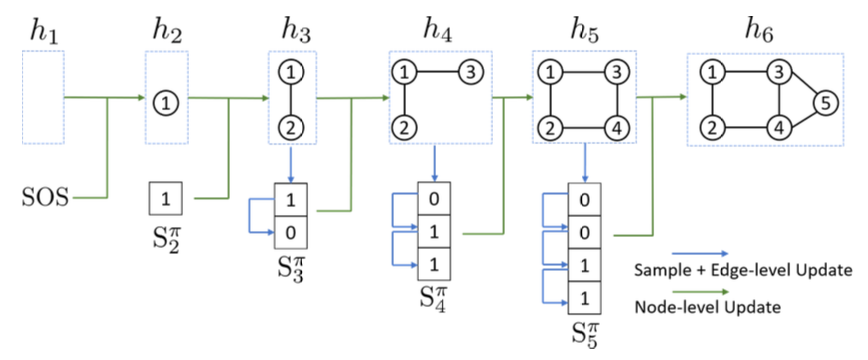
\includegraphics[scale=0.5]{graphrnn_sequences.png}
  \caption*{Figure A-1  Adjacency Vector in GraphRNN}
  \label{survey:GraphRNN}
\end{figure}

GraphRNN is based on the generation of nodes and edges, key point of
which is the estimation of \(p(S^\pi)\). Due to the sequential nature of
\(S^\pi\), we further decompose \(p(S^\pi)\) as the product of
conditional distributions over the elements:
\(p(S^\pi)=\prod\limits_{i=1}^{n+1}p(S_i^\pi|S_1^\pi, ...,S_{i-1}^\pi)\).

There are two funcitons in the calculation, a \emph{state-transition}
function \(f_{trans}\) and an \emph{output} function \(f_{out}\):

\begin{itemize}
\item
  \(f_{trans}\) is used to calculate hidden state \(h_i\) based on the
  previous hidden state and the adjacency vector,
  \(h_i=f_{trans}(h_{i-1}, S_{i-1}^\pi)\). \(h_i\in \R^d\) is a vector
  that encodes the state of the graph generated so far.
\item
  \(f_{out}\) is used to get the distribution of \(S_i^\pi\).
  \(\theta_i=f_{out}(h_i)\), \(S_i^\pi \sim \mathcal{P}_{\theta_{i}}\).
\end{itemize}

\vspace{0.2cm}

In general, \(f_{trans}\) and \(f_{out}\) can be arbitrary neural
networks, and \(\mathcal{P}_{\theta_{i}}\) can be an arbitrary
distribution over binary vectors.

\subsubsection{BFS Node-Ordering}

We can arrange the nodes to get a more effective method. So we can use
\(S^{\pi}=f_{S}(G, \operatorname{BFS}(G, \pi))\) rather than
\(S^{\pi}=f_{S}(G, \pi)\).

\(\operatorname{BFS}(G, \pi)\) means that we take a random permutation
\(\pi\) as input, picks \(π(v_1)\) as the starting node and appends the
neighbors of a node into the BFS queue in the order defined by \(\pi\).

Since the BFS function is many-to-one, \emph{i.e.}, multiple
permutations can map to the same ordering after applying the BFS
function.

There are two essential benefits:

\begin{itemize}
\item
  We only need to train on all possible BFS orderings, rather than all
  possible \(n!\) node permutations, \emph{i.e.}, multiple node
  permutations map to the same BFS ordering, providing a reduction in
  the overall number of sequences we need to consider.
\item
  The BFS ordering makes learning easier by reducing the number of edge
  predictions we need to make in the edge-level RNN; in particular, when
  we are adding a new node under a BFS ordering, the only possible edges
  for this new node are those connecting to nodes that are in the
  “frontier” of the BFS (\emph{i.e.}, nodes that are still in the BFS
  queue). In other words, if we find
  \((v_i, v_{j-1})\in E, (v_i, v_{j})\notin E, i < j \le n\), we can say
  that there are no edges between \(v_{\le i}\) and \(v_{>j}\).
\end{itemize}

\vspace{0.2cm}

\section{Dynamic Network Generation}

As far as I know, there are not such methods that can generate a dynamic
network to simulate some emergencies in the real-world. Most of the
existing methods are to split the process of graph generation into
several steps, but this will result in a series of graphs that follow
the same distribution and cannot be able to show the characteristics of
evolution.

For example, in FastSGG we can divide the generation of a single graph
into several sub-processes so that only some of the vertices are
generated in each sub-process. In most of the other methods, we can also
do such a thing to get a series of graphs.

There are also some dynamic graph generation methods based on behavior.
For example, Bob de Caux and others published a paper in 2013 \cite{De2014Dynamic}, which is based on
agent interaction behavior. The details are as follows:

\subsection{Dynamic, small-world social network generation through
local agent interactions\cite{De2014Dynamic}}

The basic idea of the model is that a network is created by collisions
between \textbf{agents} that are in “social space”. This way of
creating networks can represent many social interactions, such as
real-world person-to-person meetings and on-line meetings though social
media.

The structure of a social network can be controlled by altering
parameters of the agent's movement, such as the distance it can travel.

\subsubsection{Introduction to the Model}

So-called “social space” is a 2-dimensional space and the Euclidean
distance between any two objects will represent a social distance.

Numer of agents is fixed and agent particles are distributed randomly,
with each agent representing a potential node in the social network. The
starting point for each agent will be defined initially as the home
position and represents the point to which the agent will return after a
journey. A random angle of travel and a random range will be assigned to
each of the agents, and the range is get from a function
\(\text{agent range} =-\ln \left(\frac{x}{\lambda\left(1+\mu w_{s}\right)}\right), x\in [0,1]\).
\(w_s\) means the number of direct contacts or “neighbors”,
\(\lambda, \mu\) are fixed parameters and \(x\) is the random number
chosen to generate a range for an agent. So that we can get the target
point of the agent using the angle and the range.

From a social network viewpoint, we can view this as each agent
occupying a fixed base within the social space, from which it can
interact with others. In the model, there is a factor that the
probability of founding a connection with someone nearby in the social
space is much greater than for someone further away.

There are three stages of the movement:

\begin{itemize}
\item
  Outward movement: the agent will move to the target at a constant
  velocity. And after get there, it will reassign its target.
\item
  Homeward movement: the agent will move to its home position at a
  constant velocity. And after get there, it will reassign its target.
\item
  Post-collision movement: after colliding with another agent, the agent
  will adjust its home position. Then it will get a new target.
\end{itemize}

\vspace{0.2cm}

So-called “collision” means that two agents pass within a radius width
of each other. This will lead to the formation of the two agent nodes.

Home position of an agent \(r\) will be changed according to the
formula:
\(h_{r}^{\text {new }}=h_{r}+\boldsymbol{v}_{\boldsymbol{r s}}\left(\frac{\alpha}{\beta w_{r}+1}\right)\).
Here \(\boldsymbol{v}_{\boldsymbol{r s}}\) is the vector from \(h_r\) to
\(h_s\); \(h_r, h_s\) are the original home of the two agents of the
collision; and \(w_r\) is the number of neighbors of \(r\).
\(\alpha, \beta\) are the parameters of the system which can be seen as
a “gravity” factor. \(\beta\) is multiplied to the number of neighbors
so that it can be seen as the “local” gravity and \(\alpha\) as a
“global” gravity.

\section{Conclusion}

% These methods are from different perspectives, I have extracted the key
% ideas of the generation of them into Figures \ref{survey:Brief1} and \ref{survey:Brief2}.

These methods are from different perspectives, I have extracted the key
ideas of the generation of them into Figures A-2 and A-3.

\begin{figure}
  \label{survey:Brief1}
  \centering
  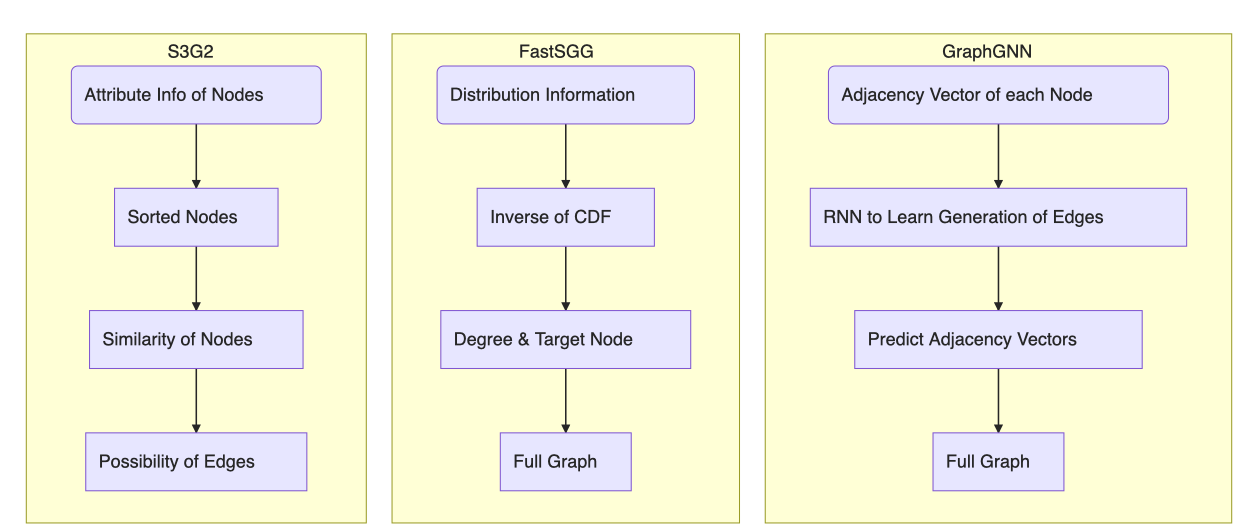
\includegraphics[scale=0.7]{image-20200514153223238.png}
  \caption*{Figure A-2  Key Ideas of S3G2, FastSGG and GraphGNN}
\end{figure}

\begin{figure}
  \label{survey:Brief2}
  \centering
  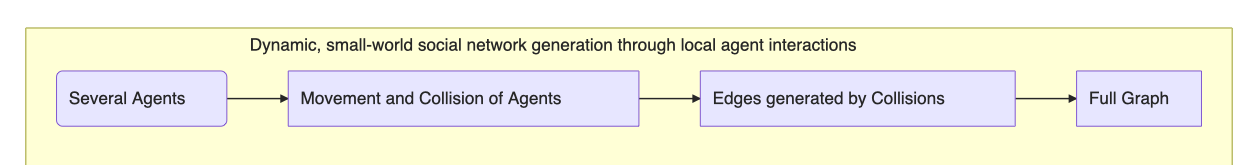
\includegraphics[scale=0.7]{image-20200514153223215.png}
  \caption*{Figure A-3  Key Idea of De2014Dynamic}
\end{figure}

I will do some research in dynamic social graph generation based on
FastSGG. Users of the generator can decide the changes over time, and
they will be able to simulate many different situations.


\bibliographystyle{plainnat}
\bibliography{ref/refs,ref/appendix}

\end{survey}
